\documentclass{standalone}
\usepackage[usenames,dvipsnames]{xcolor}
\usepackage{tikz}
\usetikzlibrary{calc}
\usetikzlibrary{arrows}
\begin{document}
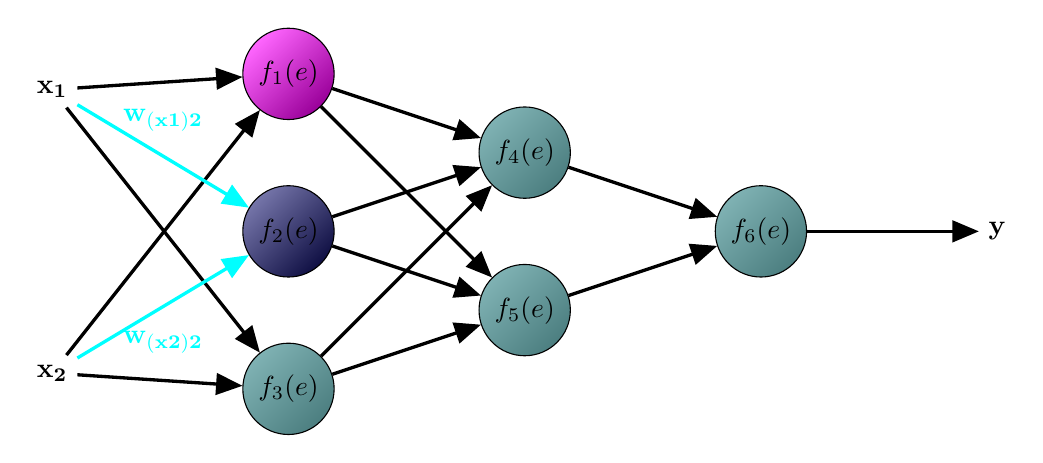
\begin{tikzpicture}
  %%Create a style for the arrows we are using
  \tikzset{normal arrow/.style={draw,-triangle 45,very thick}}
  %%Create the different coordinates to place the nodes
  \path (0,0) coordinate (1) ++(0,-2) coordinate (2) ++(0,-2) coordinate (3);
  \path (1) ++(-3,-.2) coordinate (x1);
  \path (3) ++(-3, .2) coordinate (x2);
  %%Use the calc library and partway modifiers to generate the second and third level points
  \path ($(1)!.5!(2)!3 cm!90:(2)$) coordinate (4);
  \path ($(2)!.5!(3)!3 cm!90:(3)$) coordinate (5);
  \path ($(4)!.5!(5)!3 cm!90:(5)$) coordinate (6);
  \path (6) ++(3,0) coordinate (7);
  %%Place nodes at each point using the foreach construct
  \foreach \i/\color in {1/Magenta!60,2/MidnightBlue!60,3/CadetBlue!80,4/CadetBlue!80,5/CadetBlue!80,6/CadetBlue!80}{
    \node[draw,circle,shading=axis,top color=\color, bottom color=\color!black,shading angle=45] (n\i) at (\i) {$f_{\i}(e)$};
  }
  %%Place the remaining nodes separately
  \node (nx1) at (x1) {$\mathbf{x_1}$};
  \node (nx2) at (x2) {$\mathbf{x_2}$};
  \node (ny)  at (7)  {$\mathbf{y}$};
  %%Drawing the arrows
  \path[normal arrow] (nx1) -- (n1);
  \path[normal arrow] (nx1) -- (n3);
  \path[normal arrow] (nx2) -- (n1);
  \path[normal arrow] (nx2) -- (n3);
  \path[normal arrow] (n1)  -- (n4);
  \path[normal arrow] (n1)  -- (n5);
  \path[normal arrow] (n2)  -- (n4);
  \path[normal arrow] (n2)  -- (n5);
  \path[normal arrow] (n3)  -- (n4);
  \path[normal arrow] (n3)  -- (n5);
  \path[normal arrow] (n4)  -- (n6);
  \path[normal arrow] (n5)  -- (n6);
  \path[normal arrow] (n6)  -- (ny);
  %%Drawing the cyan arrows including the labels
  \path[normal arrow,Cyan] (nx1) -- node[above=.5em,Cyan] {$\mathbf{w_{(x1)2}}$} (n2);
  \path[normal arrow,Cyan] (nx2) -- node[below=.5em,Cyan] {$\mathbf{w_{(x2)2}}$} (n2);
\end{tikzpicture}
\end{document}